\documentclass[]{article}
\usepackage{lmodern}
\usepackage{amssymb,amsmath}
\usepackage{ifxetex,ifluatex}
\usepackage{fixltx2e} % provides \textsubscript
\ifnum 0\ifxetex 1\fi\ifluatex 1\fi=0 % if pdftex
  \usepackage[T1]{fontenc}
  \usepackage[utf8]{inputenc}
\else % if luatex or xelatex
  \ifxetex
    \usepackage{mathspec}
  \else
    \usepackage{fontspec}
  \fi
  \defaultfontfeatures{Ligatures=TeX,Scale=MatchLowercase}
\fi
% use upquote if available, for straight quotes in verbatim environments
\IfFileExists{upquote.sty}{\usepackage{upquote}}{}
% use microtype if available
\IfFileExists{microtype.sty}{%
\usepackage{microtype}
\UseMicrotypeSet[protrusion]{basicmath} % disable protrusion for tt fonts
}{}
\usepackage[margin=1in]{geometry}
\usepackage{hyperref}
\hypersetup{unicode=true,
            pdftitle={Looking for evidence of a high burden of 2019-nCoV in the United States from influenza-like illness data},
            pdfauthor={Caitlin Rivers, Evan L. Ray, Nicholas G. Reich},
            pdfborder={0 0 0},
            breaklinks=true}
\urlstyle{same}  % don't use monospace font for urls
\usepackage{graphicx,grffile}
\makeatletter
\def\maxwidth{\ifdim\Gin@nat@width>\linewidth\linewidth\else\Gin@nat@width\fi}
\def\maxheight{\ifdim\Gin@nat@height>\textheight\textheight\else\Gin@nat@height\fi}
\makeatother
% Scale images if necessary, so that they will not overflow the page
% margins by default, and it is still possible to overwrite the defaults
% using explicit options in \includegraphics[width, height, ...]{}
\setkeys{Gin}{width=\maxwidth,height=\maxheight,keepaspectratio}
\IfFileExists{parskip.sty}{%
\usepackage{parskip}
}{% else
\setlength{\parindent}{0pt}
\setlength{\parskip}{6pt plus 2pt minus 1pt}
}
\setlength{\emergencystretch}{3em}  % prevent overfull lines
\providecommand{\tightlist}{%
  \setlength{\itemsep}{0pt}\setlength{\parskip}{0pt}}
\setcounter{secnumdepth}{0}
% Redefines (sub)paragraphs to behave more like sections
\ifx\paragraph\undefined\else
\let\oldparagraph\paragraph
\renewcommand{\paragraph}[1]{\oldparagraph{#1}\mbox{}}
\fi
\ifx\subparagraph\undefined\else
\let\oldsubparagraph\subparagraph
\renewcommand{\subparagraph}[1]{\oldsubparagraph{#1}\mbox{}}
\fi

%%% Use protect on footnotes to avoid problems with footnotes in titles
\let\rmarkdownfootnote\footnote%
\def\footnote{\protect\rmarkdownfootnote}

%%% Change title format to be more compact
\usepackage{titling}

% Create subtitle command for use in maketitle
\providecommand{\subtitle}[1]{
  \posttitle{
    \begin{center}\large#1\end{center}
    }
}

\setlength{\droptitle}{-2em}

  \title{Looking for evidence of a high burden of 2019-nCoV in the United States
from influenza-like illness data}
    \pretitle{\vspace{\droptitle}\centering\huge}
  \posttitle{\par}
    \author{Caitlin Rivers, Evan L. Ray, Nicholas G. Reich}
    \preauthor{\centering\large\emph}
  \postauthor{\par}
      \predate{\centering\large\emph}
  \postdate{\par}
    \date{2020-01-25 21:57:45 CET}


\begin{document}
\maketitle

\hypertarget{introduction}{%
\subsection{Introduction}\label{introduction}}

In December 2019, an outbreak of a novel, SARS-like coronavirus was
detected in Wuhan, China. In the intervening few weeks, case counts have
grown substantially. As of this writing, there are over 1200 confirmed
cases and at least 41 deaths of what is currently named 2019-nCoV
{[}1{]}. It is now understood that the virus is likely capable of person
to person spread, with a preliminary R0 estimate of 1.2 - 2.5 {[}2{]}.

Although very little sustained human to human transmission has been
observed outside of China, the possibility of unrecognized spread in
other countries cannot be ruled out at this stage. As an early effort to
explore this scenario in the United States, we compare the proportion of
weighted influenza like illness (wILI) that tests negative for influenza
during the 2019-2020 flu season to trends from previous seasons. If it
were the case that 2019-nCoV were circulating unobserved in the United
States, we might expect to see in recent weeks a higher fraction of ILI
specimens that test negative for influenza compared to the same time in
past seasons.

\hypertarget{methods}{%
\subsection{Methods}\label{methods}}

\hypertarget{data}{%
\paragraph{Data}\label{data}}

We downloaded publicly available ILINet and WHO-NREVSS data for the
national and regional levels.

From the ILINet dataset, we downloaded weighted influenza-like illness
(wILI), which measures the percentage of doctor's office visits at
sentinel providers that had the primary complaint of fever plus an
additional influenza-like symptom (cough, sore throat, etc\ldots{}). For
the WHO-NREVSS data, we obtained the total number of specimens tested by
participating clinical laboratories, as well as the percent of those
specimens that tested positive for influenza. These data have been
aggregated into a single reporting system since the 2015/2016 season, so
we use data since that time. Both data sources are available at the
weekly time-scale, defined as using the MMWR week standard used by the
CDC.

The code used to produce this report is available on GitHub at
\url{https://github.com/reichlab/ncov}.

\hypertarget{influenza-like-illness-not-attributable-to-influenza}{%
\paragraph{Influenza-like illness not attributable to
influenza}\label{influenza-like-illness-not-attributable-to-influenza}}

One possible measure of influenza illness not attributable to influenza
(ILI-) can be calculated as follows:

\[\text{ILI-} = (1 - \text{proportion of tests positive for influenza}) \times \text{wILI}\]

It is important to note that reported wILI can vary substantially due to
differences in the types of health care providers reporting into ILINet.
Therefore, some increases in reported wILI from one season to another
may be driven in part by changes in provider type make up. An
approximate way to adjust for this is by dividing reported wILI by the
baseline for a given region and season. Baselines are provided by the
CDC. This results in the following calculation of a \textbf{r}elative
ILI-.

\[\text{rILI-} = (1 - \text{proportion of tests positive for influenza}) \times \frac{\text{wILI}}{\text{baseline level for ILI}}\]

\hypertarget{results}{%
\subsection{Results}\label{results}}

We plotted ILI- and rILI- as a function of the week within each flu
season and stratified by region (Figure 1). We do not observe a strong
signal of anomalous patterns of ILI rates that are not due to influenza.
In several regions, the fraction of ILI not attributable to influenza is
near or above the highest observed rates in previous seasons, although
qualitatively it does not appear to be substantially higher than
previous years. In recent weeks, there is a trend of a lower fraction of
clinical specimens testing negative for influenza relative to wILI, but
these changes cannot be described as sustained at this time and are
still within historical norms.

Although these findings are far from conclusive, these preliminary
observations do not support a scenario of a high burden of 2019-nCoV in
the United States as of mid-January 2020.

\begin{figure}
\centering
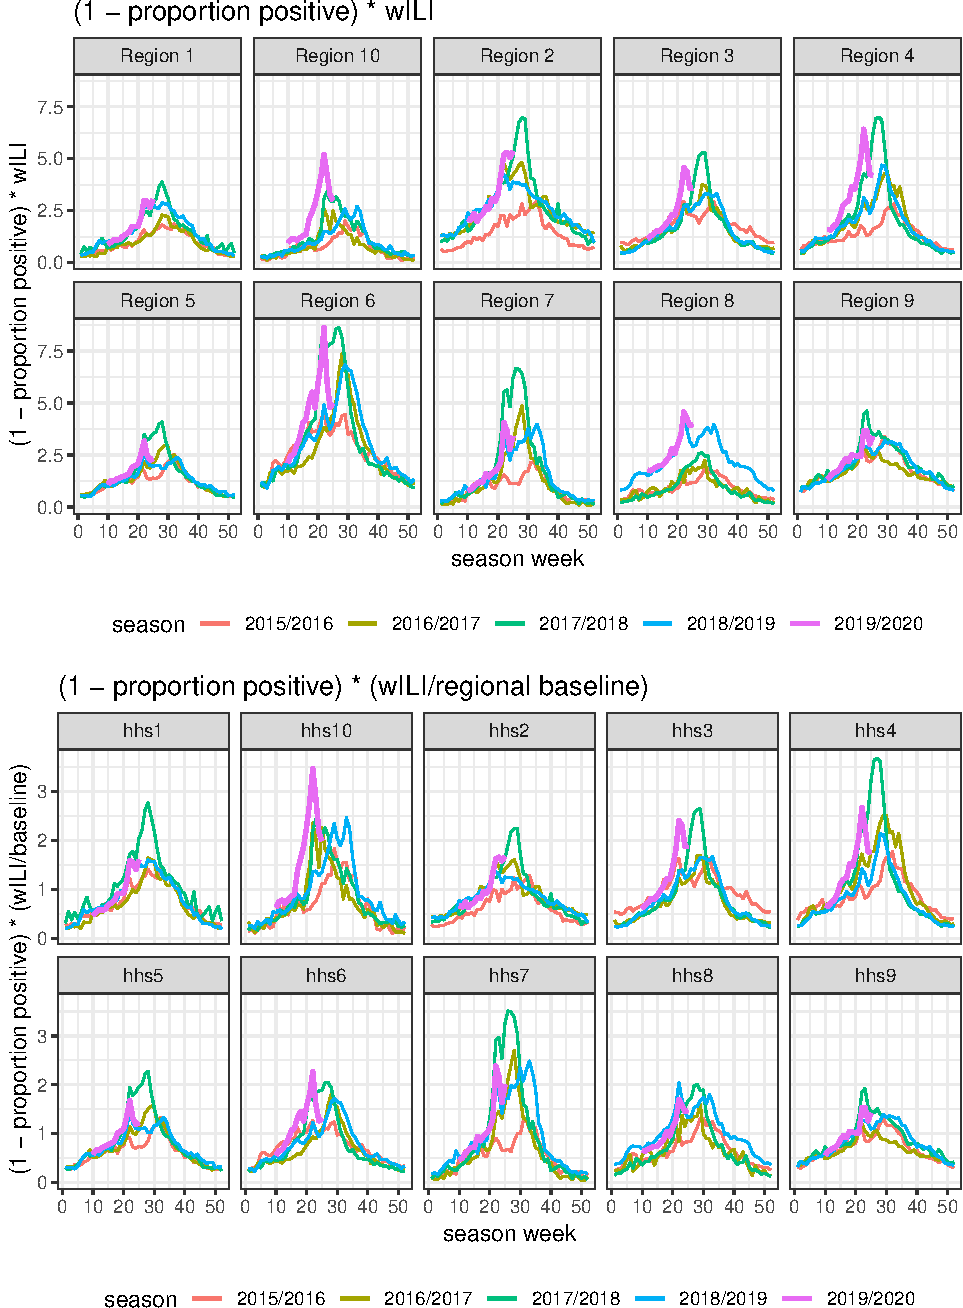
\includegraphics{ili-labtest-report_files/figure-latex/all-region-plot-ILI--1.pdf}
\caption{\label{fig:all-region-plot}US HHS Regions plots showing ILI-
values since the 2015/2016 season (top), and rILI- values (bottom).}
\end{figure}

\hypertarget{works-cited}{%
\subsection{Works Cited}\label{works-cited}}

{[}1{]}
\url{http://www.nhc.gov.cn/xcs/yqfkdt/202001/a7cf0437d1324aed9cc1b890b8ee29e6.shtml}

{[}2{]}
\url{https://www.who.int/news-room/detail/23-01-2020-statement-on-t}


\end{document}
